\documentclass[math, english, info]{beamercours}
\makeatletter
\def\tikzimp@rt{1}
\makeatother

\bibliography{slides.bib}

\usepackage{bigstrut}
\usepackage{makecell}
\usepackage{emoji}
\usepackage{tikz-dependency}
\usepackage{diag}

\def\cont{\Gamma\vdash}
\def\poulpe{\qquad}

\setlength\belowcaptionskip{0pt}
\setlength\abovecaptionskip{\baselineskip}

\DeclareMathOperator{\Var}{Var}

\def\ppl{\mathbin{+\mkern-12mu+}}

\makeatletter
\renewenvironment{thebibliography}[1]
     {\section{\bibname}
      \@mkboth{\MakeUppercase\bibname}{\MakeUppercase\bibname}%
      \list{\@biblabel{\@arabic\c@enumiv}}%
           {\settowidth\labelwidth{\@biblabel{#1}}%
            \leftmargin\labelwidth
            \advance\leftmargin\labelsep
            \@openbib@code
            \usecounter{enumiv}%
            \let\p@enumiv\@empty
            \renewcommand\theenumiv{\@arabic\c@enumiv}}%
      \sloppy
      \clubpenalty4000
      \@clubpenalty \clubpenalty
      \widowpenalty4000%
      \sfcode`\.\@m}
     {\def\@noitemerr
       {\@latex@warning{Empty `thebibliography' environment}}%
      \endlist}

\def\black@or@white#1#2{%
  \@tempdima#2 pt
  \ifdim\@tempdima>0.5 pt
    \definecolor{temp@c}{gray}{0}%
  \else
    \definecolor{temp@c}{gray}{1}%
  \fi}
\def\letterbox#1#{\protect\letterb@x{#1}}
\def\letterb@x#1#2#3{%
  \colorlet{temp@c}[gray]{#2}%
  \extractcolorspec{temp@c}{\color@spec}%
  \expandafter\black@or@white\color@spec
  {\color#1{temp@c}\tallcbox#1{#2}{#3}}}
\def\tallcbox#1#{\protect\color@box{#1}}
\def\color@box#1#2{\color@b@x\relax{\color#1{#2}}}
\long\def\color@b@x#1#2#3%
 {\leavevmode
  \setbox\z@\hbox{{\set@color#3}}%
  \ht\z@\ht\strutbox
  \dp\z@\dp\strutbox
  {#1{#2\color@block{\wd\z@}{\ht\z@}{\dp\z@}\box\z@}}}
\makeatother

\contourlength{0.005em}
\def\backbox#1{\letterbox{Lavender!40}{\contour{black}{#1}}}

\def\ty#1{\backbox{\tt\color{yulm!90!black}#1}}
\def\f#1{\backbox{\tt\color{vulm}#1}}
\def\w#1{\mathbf{#1}\,}

\def\e{\ty{e}}
\def\t{\ty{t}}
\def\r{\ty{r}}

\newcolumntype{C}{>{$}c<{$}}
\newcolumntype{L}{>{$}l<{$}}
\newcolumntype{R}{>{$}r<{$}}
\def\fmap{\texttt{fmap}}


\makeatletter
\newcommand{\@word}[4][]{%
	#2 & #3 & #4\\
\ifx&#1&%
	%
\else
	&\multicolumn{2}{l}{Generalizes to \textbf{#1}}\\%
\fi%
}
\def\word#1#2#3#4{\@word[#4]{#1}{#2}{#3}}
\makeatother

\usepackage{calc}

\makeatletter
\def\textSq#1{%
\begingroup% make boxes and lengths local
\setlength{\fboxsep}{0.4ex}% SET ANY DESIRED PADDING HERE
\setbox1=\hbox{#1}% save the contents
\setlength{\@tempdima}{\maxof{\wd1}{\ht1+\dp1}}% size of the box
\setlength{\@tempdimb}{(\@tempdima-\ht1+\dp1)/2}% vertical raise
\raise-\@tempdimb\hbox{\fbox{\vbox to \@tempdima{%
  \vfil\hbox to \@tempdima{\hfil\copy1\hfil}\vfil}}}%
\endgroup%
}
\def\Sq#1{\textSq{\ensuremath{#1}}}%

\def\c@lsep{2.3}
\def\r@wsep{.8}

\tikzset{
	uptree/.style={
			draw=green!80!black,
			thick,
		},
	typenode/.style={
			align=center,
			text width=24mm,
			%font={\large},
		},
	treenode/.style={
			align=center,
			text width=24mm,
		},
	wordnode/.style={
			inner sep=0pt,
			align=center,
			font={\large},
		},
	downtree/.style={
			draw=red!80!black,
			thick,
		},
}

\newcommand{\wnode}[3]{%
	\node (#2) at (#1*\c@lsep, 0) [wordnode] {#2};
	\node[anchor=north] (#2-) at ($(#1*\c@lsep, 0) + (0, -.142)$) [typenode] {\ensuremath{#3}};
}
\newcommand{\utnode}[3]{%
	\path let \p1 = (#2.north), \p2 = (#3.north) in coordinate (Q1) at (\x1, {max(\y1, \y2)});
	\path let \p1 = (#2.north), \p2 = (#3.north) in coordinate (Q2) at (\x2, {max(\y1, \y2)});
	\node (#2#3) at ($($(Q1)!0.5!(Q2)$) + (0, 1)$) [treenode] {\ensuremath{#1}};
	\draw[uptree] ($(#2.north) + (0, .142)$) -- (#2#3.south);
	\draw[uptree] ($(#3.north) + (0, .142)$) -- (#2#3.south);
}
\newcommand{\dtnode}[4][0.5]{%
	\path let \p1 = (#3.south), \p2 = (#4.south) in coordinate (Q1) at (\x1, {min(\y1, \y2)});
	\path let \p1 = (#3.south), \p2 = (#4.south) in coordinate (Q2) at (\x2, {min(\y1, \y2)});
	\node (#3#4) at ($($(Q1)!#1!(Q2)$) + (0, -1)$) [treenode] {\ensuremath{#2}};
	\draw[downtree] ($(#3.south) + (0, -.142)$) -- (#3#4.north);
	\draw[downtree] ($(#4.south) + (0, -.142)$) -- (#3#4.north);
}

\def\inputtikz#1{
	\ifnum\tikzimp@rt=1
		\input{figures/#1}
	\else
		\ensuremath{\text{\Huge\color{vulm}A TikZ PICTURE GOES HERE.}}
	\fi
}
\makeatother

\catstyle{catone}{gray!50}
\catstyle{catmc}{vulm!10!yulm}
\catstyle{catmca}{vulm!20!yulm}
\catstyle{catmcb}{vulm!30!yulm}
\catstyle{catmcc}{vulm!40!yulm}
\catstyle{catmcd}{vulm!50!yulm}
\catstyle{catmce}{vulm!60!yulm}
\catstyle{catmcf}{vulm!70!yulm}
\catstyle{catmcg}{vulm!80!yulm}
\catstyle{catmch}{vulm!90!yulm}

\def\din#1{#1\mathrm{.S}}
\def\dnb#1{#1\mathrm{.N}}
\def\dlb#1#2{#1\mathrm{.L}\left(#2\right)}
\def\dl#1{#1\mathrm{.L}}
\def\dnlg#1{#1\mathrm{.h}}
\def\dnin#1{#1\mathrm{.in}}
\def\dnout#1{#1\mathrm{.out}}

\newcounter{lingexcnt}
\newcounter{tmplingexcnt}
\renewcommand*{\thelingexcnt}{(\arabic{lingexcnt})}
\newenvironment{sentence}[1][]{
     \begin{list}{\thelingexcnt}{\refstepcounter{lingexcnt}}\item
     \ifnum\pdfstrcmp{#1}{}=0\else\label{#1}\fi
}{\end{list}}

\newenvironment{nsentence}{%
     \setcounter{tmplingexcnt}{\value{lingexcnt}}
     \addtocounter{tmplingexcnt}{-1}
     \begin{list}{\thelingexcnt}{
         \usecounter{lingexcnt}
         \setcounter{lingexcnt}{\value{tmplingexcnt}}
         \refstepcounter{lingexcnt}
     }
}{\end{list}}

\newcommand*{\oneSentence}[2][]{\begin{sentence}[#1]#2\end{sentence}}


\title{Effect-Driven Parsing}
\subtitle{Formal studies on a categorical approach to semantic parsing}
\institute{École Normale Supérieure | Yale University}
\addlogo{~/Pictures/Yale_University_logo.svg.png}
\addlogo{~/DEV/latex/source/ens_psl.pdf}

\begin{document}
\fancytitleframe

\section{Introduction}
\subsection{General Introduction}
\begin{frame}
	\frametitle{Salute}
	This work, based on \cite{bumfordEffectdrivenInterpretationFunctors2025} aims
	to provide a categorical formalization of a type and effects system for
	semantic interpretation of the natural language.

	\medskip

	We will develop a graphical formalism for semantic type-driven parsing that
	explains how to derive the meaning of a sentence from the meaning of its
	words.
\end{frame}

\begin{frame}[fragile]
	\frametitle{Lost in translation}
	\setcellgapes{3pt}
	\makegapedcells
	\begin{NiceTabular}{>{\bf}LLL}
		Expression & \rm Type & \lambda\text{-Term} \\
		\word{planet}{\e\to\t}{\lambda x. \w{planet} x}{common nouns}
		\word{carnivorous}{\left( \e \to \t \right)}{\lambda x. \w{carnivorous}x}{predicative adjectives}
		\word{skillful}{\left( \e \to \t \right) \to \left( \e \to \t \right)}{\lambda p. \lambda x. px \land \w{skillful} x}{predicate modifier adjectives}
		\word{Jupiter}{\e}{{\bf j}\in \Var}{proper nouns}
		\word{sleep}{\e \to \t}{\lambda x. \w{sleep} x}{intransitive verbs}
		\CodeAfter
		\begin{tikzpicture}
			\draw[double] (1|-2) -- (4|-2);
			\foreach \r in {4,6,...,10} {\draw (1|-\r) -- (4|-\r);}
		\end{tikzpicture}
	\end{NiceTabular}
\end{frame}

\begin{frame}[fragile]
	\frametitle{A, the, your}
	What should be the type of expressions such as \textbf{a cat} or \textbf{Jupiter, a planet}?
	\pause

	\smallskip

	Since we should be able to use \textbf{a cat} and \textbf{the cat} interexchangebly - from a syntax point of view - they should have the same type.
	We use \emph{effects} to do the difference between:
	\begin{equation*}
		\w{a\ cat} = \{c \mid \w{cat} c\}
	\end{equation*}
	\begin{equation*}
		\w{the\ cat} = x \text{ if } \mathbf{cat}^{-1}(\top) = \{x\} \text{ else } \#
	\end{equation*}
\end{frame}

\subsection{Just a teeny tiny bit of math}
\begin{frame}[fragile]
	\frametitle{DAMN PRINTER WHAT ARE YOU DOING}
	\begin{center}
		\begin{minipage}[b]{.45\textwidth}
			\begin{code}{python}
def add(x, y):
  return x + y
			\end{code}
			\centering
			A pure program.
		\end{minipage}
		\begin{minipage}[b]{.45\textwidth}
			\begin{code}{python}
def add(x, y):
  print("I LOVE CHOMSKY")
  return x + y
			\end{code}
			\centering
			An impure program
		\end{minipage}
	\end{center}
	\pause
	The addition of the \texttt{print} statement modifies the behaviour of the
	programs: we do not know what actually happens to the memory state of the
	computer.

	This is called a side effect, or simply effect.
\end{frame}

\begin{frame}
	\frametitle{Category Theory 101}
	\begin{itemize}
		\item A category $\mC$ is a structure with things called objects, and
		      ways to go between things called morphisms or arrows.
		      \pause
		\item Objects represent the set of objects of a certain type and arrows
		      represent ways to go from one type to another language.
		      The type of a function is then an object that represents the set
		      of arrows between $A \to B$.
	\end{itemize}
\end{frame}

\begin{frame}[fragile]
	\frametitle{Category Theory 10201}
	\begin{itemize}
		\item A functor from a category to another is a morphism between
		      categories.
		      It translates types as well as function between types.
		      \pause
		      \begin{category}
			      A\ar[r, "\phi"]\ar[d, "F"'] & B\ar[d, "F"] \\
			      FA\ar[r, "F\phi"'] & FB
		      \end{category}
		      Functors represent modifications of a type: they represent effects.
	\end{itemize}
\end{frame}

\begin{frame}[fragile]
	\frametitle{Category Theory 10202}
	\begin{itemize}
		\item A natural transformation is a morphism from a functor to another.
		      \pause
		      \begin{category}
			      FA\ar[r, "\theta_{A}"]\ar[d, "F\phi"'] & GA\ar[d, "G\phi"]\\
			      FB\ar[r, "\theta_{B}"'] & GB
		      \end{category}
	\end{itemize}
\end{frame}

\begin{frame}[fragile]
	\frametitle{Category of Endofunctors}
	\begin{itemize}
		\item A monadic effect is a type of effect that can be created from an
		      object, without losing information.
		\item When an object bears two of the same monadic effect, it can be
		      transformed to only bear one instance of the effect.
	\end{itemize}
	\pause

	Mathematically, we have two natural transformations $\eta: \Id \Rightarrow M$
	and $\mu: MM \Rightarrow M$ called unit and multiplication or join.
\end{frame}

\begin{frame}[fragile]
	\frametitle{I'm FREE! Forget it.}
	An adjunction between two functors $L \dashv R$ is a pair of natural
	transformations $\eta: \Id \Rightarrow L \circ R$ and $\epsilon: R \circ L
		\Rightarrow \Id$.

	\smallskip

	It mimics the behaviour of a bijection for functor composition.

	\pause

	A classical example is the Read - Write adjunction.
	It mimics the behaviour of the anaphora: once we have wrote data next to a
	denotation, reading said data makes us go back to the beginning, or almost.
\end{frame}

\section{Category-theoretical type system}
\subsection{Type system}
\begin{frame}
	\frametitle{Lexicon, but for the presentation}
	Let $\mL$ be our language (more on that later).
	We only suppose that our words can be applied to one another in their
	denotation system.

	\pause

	Let $\mC$ be a cartesian closed category used for typing the lexicon.
	Let $\mathcal{F}(\mL)$ be a set of functors used for representing the words
	that add an effect to our language.

	\pause\smallskip

	We consider $\bar{\mC}$ the categorical closure of $\mC$ under the action
	of $\mathcal{F}(\mL)^{*}$.
	We close it for the cartesian product and exponential of $\mC$.

	$\bar{\mC}$ represents all possible combinations of a sequence of effects
	and a base type, contains functions and products.
\end{frame}

\begin{frame}[fragile]
	\frametitle{Your honor}
	\only<1-2>{We then have typing judgements for basic combinations:
		\begin{align*}
			\only<1>{
			\frac{\cont x: \tau \poulpe \cont F \in \mathcal{F}(\mL)}{\cont Fx: F\tau }\fracnotate{Cons}                                          \\[.25cm]
			\frac{\cont x: F\tau_{1} \poulpe \cont \phi: \tau_{1} \to \tau_{2}}{\cont \phi x: F\tau_{2} }\fracnotate{\texttt{fmap}}               \\[.25cm]
				\frac{\cont x: \tau_{1} \poulpe \cont \phi: \tau_{1} \to \tau_{2}}{\cont \phi x: \tau_{2}}\fracnotate{App}
			}
			\only<2>{
			\frac{\cont x: A\tau_{1} \poulpe \cont \phi: A\left( \tau_{1} \to \tau_{2} \right)}{\cont \phi x: A\tau_{2}}\fracnotate{\texttt{<*>}} \\[.25cm]
			}
		\end{align*}
	}
	\only<3>{Typing judgements for natural transformations:
		\begin{align*}
			\frac{\cont x: \tau}{\cont x: A\tau}\fracnotate{\texttt{pure/return}} \\[.25cm]
			\frac{\cont x: MM\tau}{\cont x: M\tau}\fracnotate{\texttt{>>=}}
		\end{align*}
		More generally:
		\begin{align*}
			\forall F \overset{\theta}{\Longrightarrow} G,\poulpe \frac{\cont x: F\tau \poulpe \cont G: S' \subseteq \star \poulpe \tau \in S'}{\cont x : G\tau}\fracnotate{\texttt{nat}}
		\end{align*}
		To ensure termination and decidability, we prevent the use of the unit rule
		out of the blue, more on why that is fine later.
	}
\end{frame}

\subsection{Introducing a language}

\begin{frame}
	\frametitle{What we need}
	To present the language, we of course need the syntax of the language, as
	well as an increased model of our lexicon.
\end{frame}

\begin{frame}[fragile]
	\frametitle{What's that mean ?}
	\resizebox{\textwidth}{!}{
		\setcellgapes{3pt}
		\makegapedcells
		\begin{NiceTabular}{>{\bf}LLL}
			Expression & \rm Type & \lambda\text{-Term} \\
			\word{it}{\f{G}\e}{\lambda g. g_{0}}{}
			\word{\cdot\w{, a} \cdot}{\e \to \left(\e \to \t\right) \to \f{W}\e}{\lambda x. \lambda p. \scalar{x, p x}}{}
			\word{which}{\left( \e \to \t \right)\to \f{S}\e}{\lambda p. \left\{x \suchthat px\right\}}{}
			\word{the}{\left( \e \to \t \right) \to \f{M}\e}{\lambda p. x \text{ if } p^{-1}\left( \top \right) = \{x\} \text{ else } \#}{}
			\word{a}{\left( \e \to \t \right) \to \f{D}\e}{\lambda p. \lambda s. \left\{ \scalar{x, x \ppl s}\suchthat p x\right\}}{}
			\word{every}{\left( \e \to \t \right)\to \f{C}\e}{\lambda p. \lambda c. \forall x, px \Rightarrow cx}{}
			\CodeAfter
			\begin{tikzpicture}
				\draw[double] (1|-2) -- (4|-2);
				\foreach \r in {3,...,8} {\draw (1|-\r) -- (4|-\r);}
			\end{tikzpicture}
		\end{NiceTabular}
	}
\end{frame}

\begin{frame}
	\frametitle{Independence}
	\only<1-2>{Using the notion of functors, we can also implement higher-order semantic
		constructions in our lexicon, such as the future, without caring about
		morphological markers:}
	\only<2>{%
		\begin{equation*}
			\columneqs{
				\bf future\left(be\left( I, a\ cat \right)\right)
				\xrightarrow{\beta} be\left( future\left( I \right), a\ cat \right)
				\xrightarrow{\beta} be\left( future\left( I \right), a\ cat \right)
			}
		\end{equation*}
		Those constructs are integrated by using natural transformations explaining
		their propagation through other effects, as those are purely
		semantic predicates.
	}
	\only<3>{
		For the plural, this gives:
		\resizebox{\textwidth}{!}{%
			\def\arraystretch{1.3}
			\setcellgapes{3pt}
			\makegapedcells
			\begin{NiceTabular}{>{\bf}c>{\cont}C>{\Pi(p) = }L}
				CN(P)                       & p: \left(\e \to \t\right)                                & \lambda x.\left( px \land \abs{x} \geq 2 \right)                                                \\
				\multirow{2}{*}{\bf ADJ(P)} & p: \left( \e \to \t \right)                              & \lambda x. \left( px \land \abs{x} \geq 2 \right)                                               \\
				                            & p: \left( \e \to \t \right) \to \left( \e \to \t \right) & \lambda \nu. \lambda x. \left( p\left( \nu \right)\left( x \right) \land \abs{x} \geq 2 \right) \\
				\multirow{2}{*}{\bf NP}     & p: \e                                                    & p                                                                                               \\
				                            & p: \left( \e \to \t \right) \to \t                       & \lambda \nu. p\left( \Pi \nu \right)                                                            \\
				IV(P)/VP                    & p: \e \to \t                                             & \lambda o. \left( po \land \abs{x} \geq 2 \right)                                               \\
				TV(P)                       & p: \e \to \e \to \t                                      & \lambda s. \lambda o. \left( p\left( s \right)\left( o \right) \land \abs{s} \geq 2 \right)     \\
				\CodeAfter
				\begin{tikzpicture}
					\foreach \r in {2,...,7} {\draw[dashed] ($(2|-\r) + (.1, 0)$) -- (4|-\r);}
					\foreach \r in {2, 4, 6, 7} {\draw (1|-\r) -- (4|-\r);}
				\end{tikzpicture}
			\end{NiceTabular}
		}
	}
	\only<4>{
	}
\end{frame}

\section{Effect Handling}
\subsection{What is a chair ?}
\begin{frame}
	\frametitle{Q}
	A handler for an effect $F$ is a natural transformation $F \Rightarrow \Id$.

	\smallskip

	Handlers should also be exact inverses to monadic and applicative units:
	this justifies semantically why we can remove the usage of the unit rule out
	of certain situations.
\end{frame}


\begin{frame}
	\frametitle{Alphabetical philosophy}
	There are two main types of handlers that are of interest to us:
	\pause
	\begin{enumerate}
		\item Language-Defined Handlers, which are defined with
		      adjunctions and comonads, for example.
		      Those arise from fundamental properties of the considered effects.
		      \pause
		\item Speaker-dependant handlers, which are considered when
		      retrieving the denotation from a sentence from under the effects
		      that arose in the computation of its meaning.
		      Those need to be considered dependent on the speaker because for
		      example of the multiple ways to solve non-determinism.
	\end{enumerate}
\end{frame}
\begin{frame}
	\frametitle{Friday}
	The notion of handlers allows us to enforce the notion of scope islands.
	To do so, it would suffice to ask that the words enclosing the island,
	are not defined on not certain effectful types and make handlers a part of
	the combination modes.

	\pause
	\smallskip

	We would for example have:
	\begin{equation*}
		\w{if}: \left(\t \setminus \mF{\mL}^{*}\f{C}\t \right) \to \t \to \t
	\end{equation*}

\end{frame}
\subsection{The ropes of effect handling.}
\begin{frame}[allowframebreaks]
	\frametitle{Pantone}
	A string diagram is a representation of the side-effects and types of a
	sentence across its computation.

	\begin{center}
		\begin{minipage}[c]{.45\textwidth}
			\inputtikz{sd-thecatsleeps}
		\end{minipage}
    \begin{minipage}[c]{.45\textwidth}
      This diagram for example represents the sentence \textsl{The cat sleeps}.
    	The order of the words and position of the strings will be explained in
    	detail in the next section.
    \end{minipage}
	\end{center}

\end{frame}

\subsection{Severing the ties.}
\begin{frame}
	\frametitle{Tying the knots}
	String diagrams will be the formalism we use to compute equality between
	denotations, and especially handling the denotations.
	\begin{thm}[Theorem 3.1 \cite{selingerSurveyGraphicalLanguages2010}, Theorem 1.2 \cite{joyalGeometryTensorCalculus1991}]
		\label{thm:isotopy}
		A well-formed equation between morphism terms in the language of monoidal
		categories follows from the axioms of monoidal categories if and only if it
		holds, up to planar isotopy, in the graphical language.
	\end{thm}
\end{frame}

\begin{frame}[allowframebreaks]
	\frametitle{Version 7.0.}
	Every property of the functors, monads, natural transformations, adjunctions
	and more can be explained in terms of commutative diagrams, but also as
	string diagrams.

	First, the elevator equations are a consequence of \ref{thm:isotopy}:
	\begin{equation}
		\resizebox{.8\textwidth}{!}{\inputtikz{sd-elevator}}
		\label{eq:elevator}
		\tag{\href{https://î.fr/ascenseurs}{\emoji{elevator}}}
	\end{equation}

	The Snake equations are a rewriting of the properties of an adjunction:
	\begin{equation}
		\resizebox{.5\textwidth}{!}{\inputtikz{sd-snake1}}
		\tag{\rotatebox[origin=c]{90}{\emoji{snake}}}
		\label{eq:snek1}
	\end{equation}

	The Monadic equations are a rewriting of the properties of a monad:
	\begin{equation}
		\resizebox{.5\textwidth}{!}{\inputtikz{sd-monad-mult}}
		\label{eq:muax}
		\tag{$\mu$}
	\end{equation}

\end{frame}

\begin{frame}[allowframebreaks]
	\frametitle{Bubba Gump Shrimps}
	\begin{thm}[Confluence]\label{thm:confluence}
		Our reduction system is confluent and therefore defines normal forms:
		\begin{enumerate}
			\item Right reductions are confluent and therefore define \emph{right} normal forms for
			      diagrams under the equivalence relation induced by exchange.
			\item Equational reductions are confluent and therefore define \emph{equational}
			      normal forms for diagrams under the equivalence relation induced by exchange.
		\end{enumerate}
	\end{thm}

	\smallskip

	\begin{thm}[Normalization Complexity]
		\label{thm:normalize}
		Reducing a diagram to its normal form is done in quadratic time in
		the number of natural transformations in it.
	\end{thm}
	This is accomplished using a formalism based on \cite{delpeuchNormalizationPlanarString2022}.
\end{frame}

\section{Semantic Parsing}
\subsection{Actor's studio}
\begin{frame}[allowframebreaks]
	\frametitle{Chomsky did nothing wrong.}
	We use a Context-Free Grammar to model our typing system and take its product with the syntax defining grammar.

	\begin{minipage}{\textwidth}
		\small
		\begin{multicols}{2}
			\def\arraystretch{1.2}
			\begin{mgrammar}
				\gskip
				\firstrule{>, \beta}{\left(\alpha\to \beta\right), \alpha}{}
				\firstrule{<, \beta}{\alpha, \left(\alpha \to \beta\right)}{}
				\firstrule{\wedge, \alpha \to \t}{\left(\alpha \to \t\right), \left(\alpha \to \t\right)}{}
				\firstrule{\vee, \alpha \to \t}{\left(\alpha \to \t\right), \left(\alpha \to \t\right)}{}
				\gskip
				\firstrule{\combJ_{\f{F}}\  \f{F}\tau}{\f{F}\f{F}\tau}{}
				\firstrule{\combDN_{\f{C}}\  \tau}{\f{C}_{\tau}\tau}{}
				\gskip
			\end{mgrammar}

			\def\arraystretch{1.3}
			\begin{mgrammar}
				\firstrule{\combML_{\f{F}} \left(\alpha, \beta\right)}{\f{F}\alpha, \beta}{}
				\firstrule{\combMR_{\f{F}} \left(\alpha, \beta\right)}{\alpha, \f{F}\beta}{}
				\firstrule{\combA_{\f{F}} \left(\alpha, \beta\right)}{\f{F}\alpha, \f{F}\beta}{}
				\firstrule{\combUR_{\f{F}} \left(\alpha \to \alpha', \beta\right)}{\f{F}\alpha\to \alpha', \beta}{}
				\firstrule{\combUL_{\f{F}} \left(\alpha, \beta\to \beta'\right)}{\alpha, \f{F}\beta \to \beta'}{}
				\firstrule{\combC_{\f{L}\f{R}} \left(\f{L} \alpha, \f{R}\beta\right)}{\left(\alpha, \beta\right)}{}
				\firstrule{\combER_{\f{R}} \left(\f{R}\left(\alpha \to \alpha'\right), \beta\right)}{\alpha\to \f{R}\alpha', \beta}{}
				\firstrule{\combEL_{\f{R}} \left(\alpha, \f{R}\left(\beta \to \beta'\right)\right)}{\alpha, \beta\to \f{R}\beta'}{}
			\end{mgrammar}
		\end{multicols}
	\end{minipage}

	\smallskip

	This grammar works in five major sections:
	\begin{enumerate}
		\item We reintroduce the grammar defining the type and effect system.
		\item We introduce a structure for the semantic parse trees and their labels,
		      the combination modes from
		      \cite{bumfordEffectdrivenInterpretationFunctors2025}.
		\item We introduce rules for basic type combinations.
		\item We introduce rules for higher-order unary type combinators.
		\item We introduce rules for higher-order binary type combinators.
	\end{enumerate}
\end{frame}

\begin{frame}[allowframebreaks, fragile]
	\frametitle{Where cats are stuck.}
	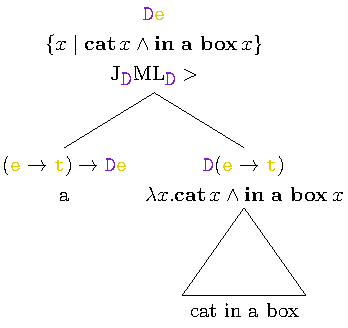
\includegraphics{aux/figures/parse-tree-1.pdf}
	\centering
	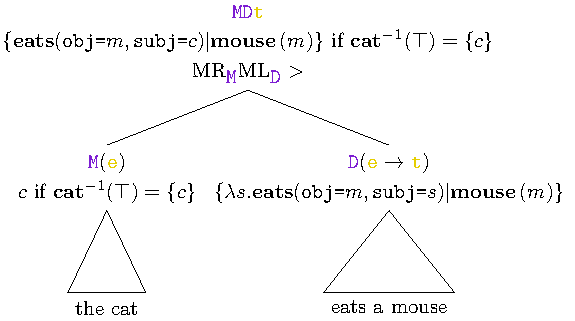
\includegraphics{aux/figures/parse-tree-2.pdf}

	{\centering 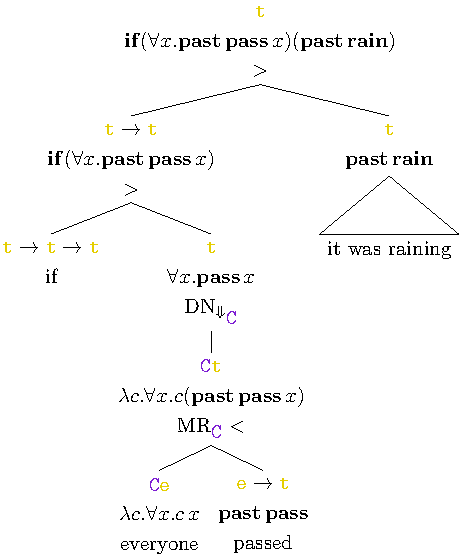
\includegraphics[height=.7\pageheight]{aux/figures/parse-tree-3.pdf}}
\end{frame}


\subsection{No strings attached.}
\begin{frame}
	\frametitle{Legos, with strings}
	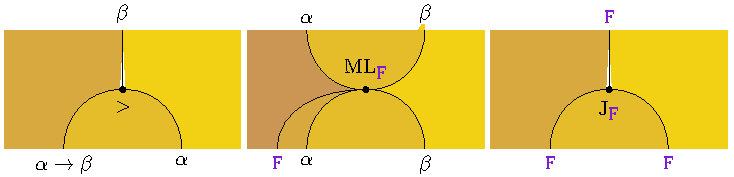
\includegraphics[width=\textwidth]{aux/figures/combinators-sd.pdf}
\end{frame}

\begin{frame}
	\frametitle{Crayons}
	Based on the mathematical definitions of the combinators, we can also define
	reduction rules as a part of the grammar (and later, on our string diagrams).

	This allows us to reduce the grammar while still using the properties of
	string diagrams to our advantage in the proofs.
\end{frame}

\begin{frame}
	\frametitle{Under the old willow}
	\rotatebox{-90}{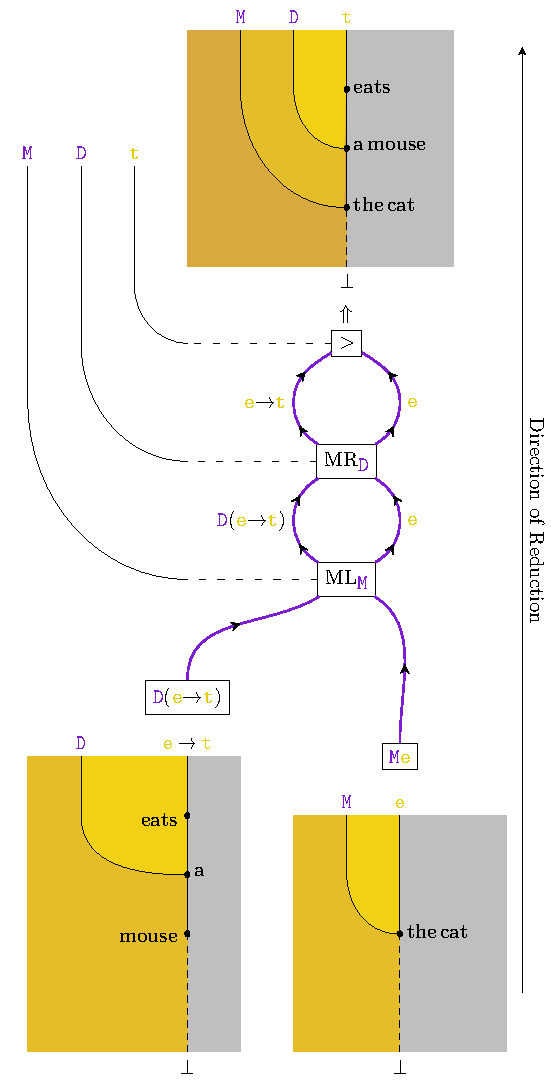
\includegraphics[height=\textwidth]{aux/figures/parsing-diagram.pdf}}
\end{frame}

\begin{frame}
	\frametitle{Under the older willow}
	\rotatebox{-90}{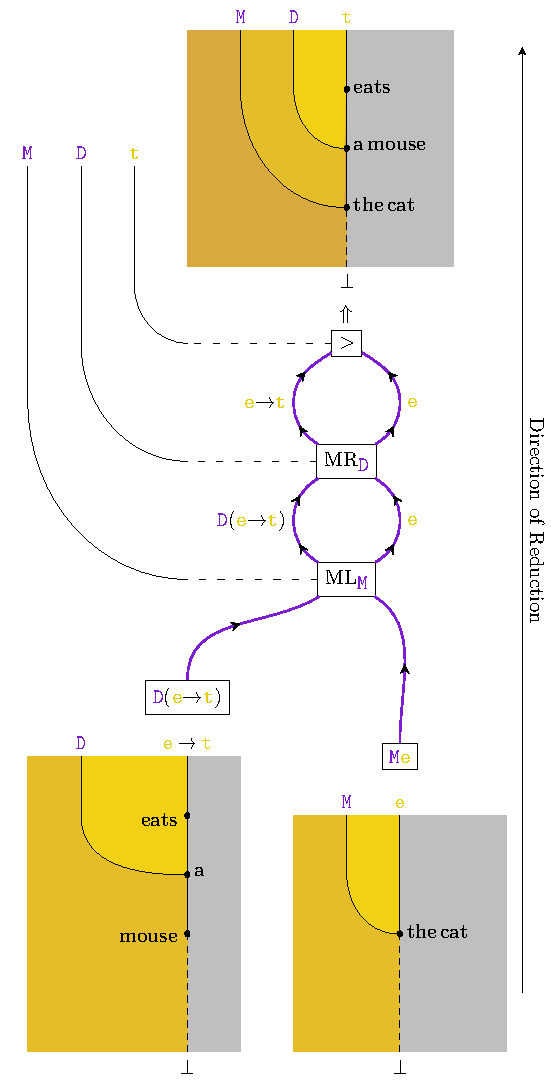
\includegraphics[height=\textwidth]{aux/figures/parsing-diagram.pdf}}
\end{frame}

\begin{frame}
	\frametitle{Knitting with words}
	\centering
	
\includegraphics[width=.7\textwidth]{aux/figures/knitting-example.jpeg}
\end{frame}

\begin{frame}
	\frametitle{Willows, but better!}
	\vspace{-.25cm}
	\centering
	\rotatebox{-90}{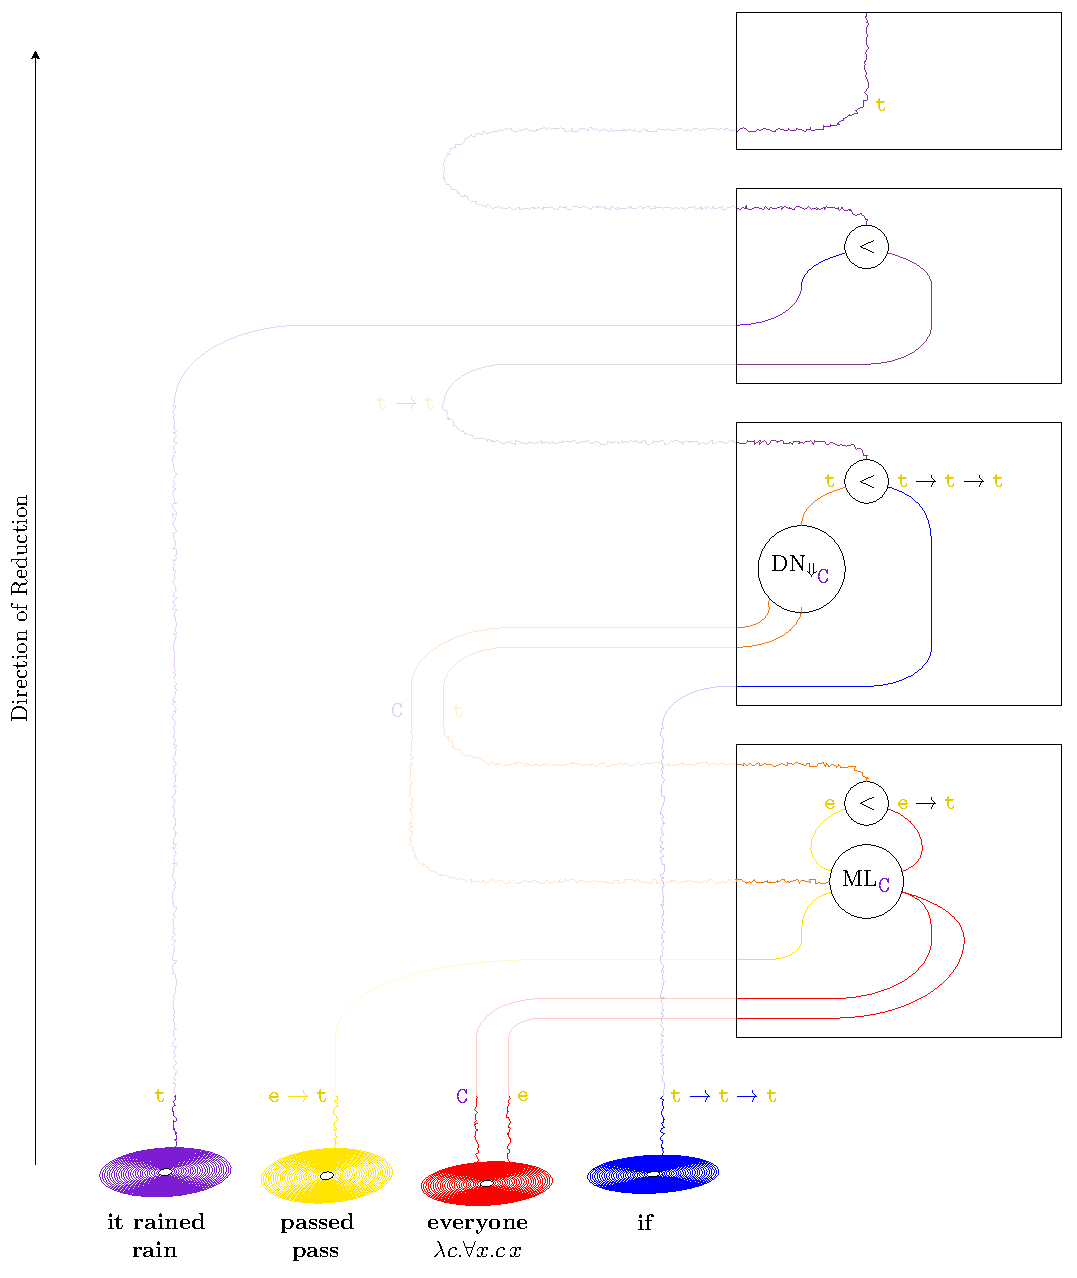
\includegraphics[width=.7\pageheight]{aux/figures/3d-parsing-diagram.pdf}}
\end{frame}

\end{document}

